%%%%%%%%%%%%%%%%%%%%%%%%%%%%%%%%%%%%%%%%%%%%%%%%%%%%%%%%%%%%%%%%%%%%%%%%%%%%%%%%%%%%%%%%%%%%%%%%%%%%%%%%%%%%%%%
\chapter{Přehled parametrů jednotlivých jednodeskových počítačů}
\label{PrilohaTabulka}
	\colorbox[rgb]{1,0,0}{doresit: otocit o 90? mozna hodit na A3?}
\begin{table}[!ht]
\centering
\caption{Přehled parametrů jednotlivých jednodeskových počítačů}
\label{PrilohaTabulkaTabulka}
\resizebox{\textwidth}{!}{
\begin{tabular}{|l|l|l|l|l|l|l|l|l|l|l|l|l|l|l|l|l|l|l|l|l|l|l|l|l|l|l|}
\hline
\textbf{Označení modulu} &  & \textbf{Mikrokontrolér} & \textbf{Platforma} & \textbf{Rozlišení {[}b{]}} & \textbf{Frekvence {[}MHz{]}} & \textbf{Flash {[}KiB{]}} & \textbf{EEPROM {[}KiB{]}} & \textbf{SRAM {[}KiB{]}} & \textbf{Digitální piny} & \textbf{PWM kanály} & \textbf{Analogové vstupy} & \textbf{UART sběrnice} & \textbf{I2C sběrnice} & \textbf{SPI sběrnice} & \textbf{Ethernet} & \textbf{Wifi} & \textbf{USB master} & \textbf{MicroSD} & \textbf{Mini PCIe} & \textbf{SATA} & \textbf{Grafický výstup} & \textbf{Bluetooth} & \textbf{HDMI} & \textbf{Podpora shieldů} & \textbf{USB rozhraní} & \textbf{Rozměry} \\ \hline
Arduino & \textbf{Diecimila} & ATmega168 &  &  &  & 16 & 0.5 & 1 & 14 & 6 & 6 & ano & ano & ano &  &  &  &  &  &  &  &  &  & ano & FTDI & 68.6mm x 53.3mm \\ \hline
 & \textbf{Duemilanove} & ATmega168 &  &  &  & 16 & 0.5 & 1 & 14 & 6 & 6 & ano & ano & ano &  &  &  &  &  &  &  &  &  & ano & FTDI & 68.6mm x 53.3mm \\ \hline
 & \textbf{} & ATmega328P &  &  &  & 32 & 1 & 2 & 14 & 6 & 6 & ano & ano & ano &  &  &  &  &  &  &  &  &  & ano & FTDI & 68.6mm x 53.3mm \\ \hline
 & \textbf{Uno} & ATmega328P &  &  &  & 32 & 1 & 2 & 14 & 6 & 6 & ano & ano & ano & - & - & - & - &  &  &  & - &  & ano & ATmega8U2 & 68.6mm x 53.3mm \\ \hline
 & \textbf{Due} & ATMEL SAM3U &  &  &  & 256 & - & 50 & - & - & 16 & ano & ano & ano &  &  &  &  &  &  &  &  &  & ano &  & 101.52 x 53.3mm \\ \hline
 & \textbf{Mega} & ATmega1280 &  &  &  & 128 & 4 & 8 & 54 & 14 & 16 & ano & ano & ano &  &  &  &  &  &  &  &  &  & ano & FTDI & 101.6mm x 53.3mm \\ \hline
 & \textbf{Mega2560} & ATmega2560 &  &  &  & 256 & 4 & 8 & 54 & 14 & 16 & ano & ano & ano &  &  &  &  &  &  &  &  &  & ano & ATmega8U2 & 101.6mm x 53.3mm \\ \hline
 & \textbf{Leonardo} & ATmega32u4 &  &  &  & 32 & 1 & 2 & 14 & 6 & 12 &  &  &  &  &  &  &  &  &  &  &  &  &  & Atmega32u4 & 68.6mm × 53.3mm \\ \hline
 & \textbf{Fio} & ATmega328P &  &  &  & 32 & 1 & 2 & 14 & 6 & 8 &  &  &  &  &  &  &  &  &  &  &  &  &  & - & 40.6mm x 27.9mm \\ \hline
 & \textbf{Mini} &  &  &  &  &  &  &  &  &  &  &  &  &  &  &  &  &  &  &  &  &  &  &  &  &  \\ \hline
 & \textbf{Micro} &  &  &  &  &  &  &  &  &  &  &  &  &  &  &  &  &  &  &  &  &  &  &  &  &  \\ \hline
 & \textbf{Nano v1} & ATmega168 &  &  &  & 16 & 0.5 & 1 & 14 & 6 & 8 &  &  &  &  &  &  &  &  &  &  &  &  &  & FTDI & 43mm x 18mm \\ \hline
 & \textbf{Nano v2} & ATmega328 &  &  &  & 32 & 1 & 2 & 14 & 6 & 8 &  &  &  &  &  &  &  &  &  &  &  &  &  & FTDI & 43mm x 18mm \\ \hline
 & \textbf{LilyPad} & ATmega168V &  &  &  & 16 & 0.5 & 1 & 14 & 6 & 6 &  &  &  &  &  &  &  &  &  &  &  &  &  & - & ø 50mm \\ \hline
 & \textbf{LilyPad} & ATmega328V &  & 8 & 8 & 16 & 0.5 & 1 & 14 & 6 & 6 &  &  &  &  &  &  &  &  &  &  &  &  &  & - & ø 50mm \\ \hline
 & \textbf{Ýun} & Atheros AR9331 &  &  & 400 & 16 MiB & 1 & 64 MiB & - & 7 & 12 & ano & ano & ano & ano & ano & ano & ano &  &  &  & - &  & ano & Atmega32u4 & 68.6mm x 53.3mm \\ \hline
 & \textbf{} & ATmega32u4 &  &  & 16 & 32 &  & 1 &  &  &  &  &  &  &  &  &  &  &  &  &  &  &  &  &  &  \\ \hline
Arduino klony & \textbf{Teensy 2.0} & ATMEGA32U4 &  & 8 & 16 & 32 &  &  &  &  &  &  &  &  &  &  &  &  &  &  &  &  &  &  &  &  \\ \hline
 & \textbf{Teensy++ 2.0} & AT90USB1286 &  & 8 & 16 & 128 &  &  &  &  &  &  &  &  &  &  &  &  &  &  &  &  &  &  &  &  \\ \hline
 & \textbf{Teensy 3.0} & MK20DX128 & ARM & 32 & 48 & 128 &  &  &  &  &  &  &  &  &  &  &  &  &  &  &  &  &  &  &  &  \\ \hline
 & \textbf{Teensy 3.1} & MK20DX256 & ARM & 32 & 72 & 256 &  &  &  &  &  &  &  &  &  &  &  &  &  &  &  &  &  &  &  &  \\ \hline
 & \textbf{Freeduino} &  &  &  &  &  &  &  &  &  &  &  &  &  &  &  &  &  &  &  &  &  &  &  &  &  \\ \hline
 & \textbf{LABduino} &  &  &  &  &  &  &  &  &  &  &  &  &  &  &  &  &  &  &  &  &  &  &  &  &  \\ \hline
 & \textbf{Arduelo Libero} &  &  &  &  &  &  &  &  &  &  &  &  &  &  &  &  &  &  &  &  &  &  &  &  &  \\ \hline
 & \textbf{Bare Bones Board} &  &  &  &  &  &  &  &  &  &  &  &  &  &  &  &  &  &  &  &  &  &  &  &  &  \\ \hline
 & \textbf{Runtime} &  &  &  &  &  &  &  &  &  &  &  &  &  &  &  &  &  &  &  &  &  &  &  &  &  \\ \hline
 & \textbf{Nanode} &  &  &  &  &  &  &  &  &  &  &  &  &  &  &  &  &  &  &  &  &  &  &  &  &  \\ \hline
 & \textbf{Freakduino} &  &  &  &  &  &  &  &  &  &  &  &  &  &  &  &  &  &  &  &  &  &  &  &  &  \\ \hline
 & \textbf{Seeeeduino} &  &  &  &  &  &  &  &  &  &  &  &  &  &  &  &  &  &  &  &  &  &  &  &  &  \\ \hline
 & \textbf{Diavolino} &  &  &  &  &  &  &  &  &  &  &  &  &  &  &  &  &  &  &  &  &  &  &  &  &  \\ \hline
 & \textbf{Boarduino} &  &  &  &  &  &  &  &  &  &  &  &  &  &  &  &  &  &  &  &  &  &  &  &  &  \\ \hline
Intel & \textbf{Galileo} & Intel Quark X1000 & x86 & 12 & 400 & 8 MB & 8 & 256MB & 14 & 6 & 6 & ano & ano & ano & ano & - & ano & ano & ano & - & - & - &  & ano &  &  \\ \hline
 & \textbf{Edison} & Intel Quark & x86 & 12 & 400 & 4 GB & 8 & 1 GB & 20 & 4 & 6 & ano & ano & ano & - & ano & ano & ano & - & - & - & ano &  & ano &  & 35.5 x 25 x 3.9 mm \\ \hline
AMD & \textbf{Gizmo} & AMD GX210HA & amd64 &  & 1GHz & - &  & 1GB & ano & ano & ano & ano & ano & ano & ano & - & ano & ano & - & ano & ano & - &  & - &  & 101.6 x 101.6 mm \\ \hline
 & \textbf{Gizmo 2} &  & amd64 &  & 1GHz & - &  & 1GB & ano & ano & ano & ano & ano & ano & ano & - & ano & ano & - & ano & ano & - &  & - &  & 101.6 x 101.6 mm \\ \hline
Raspberry & \textbf{Raspbery Pi A} &  &  &  &  &  &  &  &  &  &  &  &  &  &  &  &  &  &  &  &  &  &  &  &  &  \\ \hline
 & \textbf{Raspbery Pi B} &  &  &  &  &  &  &  &  &  &  &  &  &  &  &  &  &  &  &  &  &  & ano &  &  &  \\ \hline
 & \textbf{Raspbery Pi +} &  &  &  &  &  &  &  &  &  &  &  &  &  &  &  &  &  &  &  &  &  & ano &  &  &  \\ \hline
 & \textbf{Raspbery Pi 2} &  &  &  &  &  &  &  &  &  &  &  &  &  &  &  &  &  &  &  &  &  &  &  &  &  \\ \hline
 & \textbf{Raspbery Pi 3} &  &  &  &  &  &  &  &  &  &  &  &  &  &  &  &  &  &  &  &  &  &  &  &  &  \\ \hline
 & \textbf{Raspbery Pi Zero} &  &  &  &  &  &  &  &  &  &  &  &  &  &  &  &  &  &  &  &  &  &  &  &  &  \\ \hline
Raspberry klony & \textbf{Banana Pi} &  &  &  &  &  &  &  &  &  &  &  &  &  &  &  &  &  &  &  &  &  &  &  &  &  \\ \hline
 & \textbf{OrangePi} &  &  &  &  &  &  &  &  &  &  &  &  &  &  &  &  &  &  &  &  &  &  &  &  &  \\ \hline
 & \textbf{CubieBoard} &  &  &  &  &  &  &  &  &  &  &  &  &  &  &  &  &  &  &  &  &  &  &  &  &  \\ \hline
 & \textbf{UpBoard} &  &  &  &  &  &  &  &  &  &  &  &  &  &  &  &  &  &  &  &  &  &  &  &  &  \\ \hline
 & \textbf{PINE64} &  &  &  &  &  &  &  &  &  &  &  &  &  &  &  &  &  &  &  &  &  &  &  &  &  \\ \hline
 & \textbf{HardKernel Odroid} &  &  &  &  &  &  &  &  &  &  &  &  &  &  &  &  &  &  &  &  &  &  &  &  &  \\ \hline
 & \textbf{BeagleBoard} &  &  &  &  &  &  &  &  &  &  &  &  &  &  &  &  &  &  &  &  &  &  &  &  &  \\ \hline
\end{tabular}}
\end{table}




%%%%%%%%%%%%%%%%%%%%%%%%%%%%%%%%%%%%%%%%%%%%%%%%%%%%%%%%%%%%%%%%%%%%%%%%%%%%%%%%%%%%%%%%%%%%%%%%%%%%%%%%%%%%%%%
\chapter{Ukázka zachycených dat}
\label{PrilohaVystup}
	\colorbox[rgb]{1,0,0}{bude update}
	\begin{lstlisting}[style=MyCodeBash]
		Device is on AMA0: True
		Device is waked up: True
		Device is set as Sniffer T: <OK
		Sniffing now:

		05:32:43 10/12/2016    Senzor: WEP.1b.00000010.02    Teplota: 44.8C    Vlhkost:  7.9%      RSSI:  -73dBm      Mereni: 56
		05:33:42 10/12/2016    Senzor: WEP.1b.00000010.02    Teplota: 44.7C    Vlhkost:  7.3%      RSSI:  -65dBm      Mereni: 57
		05:34:40 10/12/2016    Senzor: WEP.1b.00000010.02    Teplota: 44.8C    Vlhkost:  6.2%      RSSI:  -81dBm      Mereni: 58
		...
		20:32:43 11/12/2016    Senzor: WEP.1b.00000010.02    Teplota: 19.8C    Vlhkost: 34.9%      RSSI:  -70dBm      Mereni: 107
		20:33:42 11/12/2016    Senzor: WEP.1b.00000010.02    Teplota: 19.8C    Vlhkost: 34.3%      RSSI:  -57dBm      Mereni: 108
		20:34:40 11/12/2016    Senzor: WEP.1b.00000010.02    Teplota: 19.8C    Vlhkost: 34.2%      RSSI:  -64dBm      Mereni: 109
		...
		12:22:10 12/12/2016    Senzor: WEP.1b.00000010.02    Teplota: -2.7C    Vlhkost: 61.6%      RSSI: -104dBm      Mereni: 182
		12:23:09 12/12/2016    Senzor: WEP.1b.00000010.02    Teplota: -2.7C    Vlhkost: 61.1%      RSSI: -108dBm      Mereni: 183 
		12:24:08 12/12/2016    Senzor: WEP.1b.00000010.02    Teplota: -2.8C    Vlhkost: 61.4%      RSSI:  -93dBm      Mereni: 184
		...
		09:52:17 13/12/2016    Senzor: WEP.1b.00000010.02    Teplota: 14.3C    Vlhkost: 39.6%      RSSI:  -34dBm      Mereni: 2
		09:53:16 13/12/2016    Senzor: WEP.1b.00000010.02    Teplota: 13.4C    Vlhkost: 38.1%      RSSI:  -28dBm      Mereni: 3 
		09:54:18 13/12/2016    Senzor: WEP.1b.00000010.02    Teplota: 13.8C    Vlhkost: 37.4%      RSSI:  -33dBm      Mereni: 4
		...
		17:45:07 14/12/2016    Senzor: WEP.1b.00000010.02    Teplota: 25.7C    Vlhkost: 30.9%      RSSI:  -91dBm      Mereni: 165
		17:46:07 14/12/2016    Senzor: WEP.1b.00000010.02    Teplota: 25.7C    Vlhkost: 31.2%      RSSI:  -84dBm      Mereni: 166
		17:47:06 14/12/2016    Senzor: WEP.1b.00000010.02    Teplota: 25.8C    Vlhkost: 31.7%      RSSI:  -96dBm      Mereni: 167

	\end{lstlisting}
	
%%%%%%%%%%%%%%%%%%%%%%%%%%%%%%%%%%%%%%%%%%%%%%%%%%%%%%%%%%%%%%%%%%%%%%%%%%%%%%%%%%%%%%%%%%%%%%%%%%%%%%%%%%%%%%%
\chapter{Ukázka vizualizace dat}
\label{PrilohaGrafy}
	\colorbox[rgb]{1,0,0}{tady budou grafy}
	 \begin{figure}[!ht]
  \begin{center}
    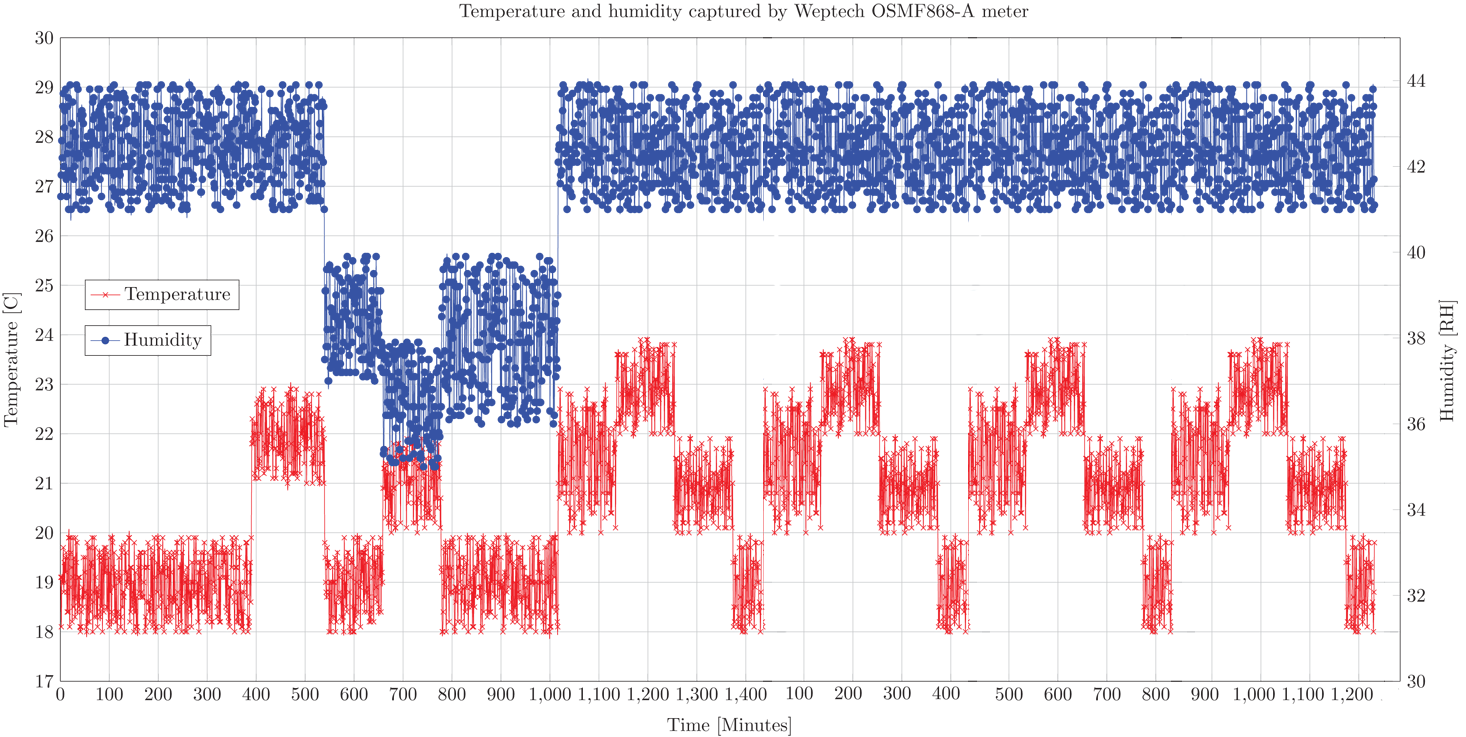
\includegraphics[scale=0.8]{obrazky/chart_weptech}
  \end{center}
  \caption{Ukazka vizualizace dat}
	\label{GrafPriloha1}
\end{figure}

%%%%%%%%%%%%%%%%%%%%%%%%%%%%%%%%%%%%%%%%%%%%%%%%%%%%%%%%%%%%%%%%%%%%%%%%%%%%%%%%%%%%%%%%%%%%%%%%%%%%%%%%%%%%%%%
\chapter{Obsah přiloženého DVD}
\label{PrilohaMedium}
K diplomové práci je přiloženo CD, obsahující bitový obraz MicroSD karty se systémem Raspbian, ve kterém je nainstalováno a nastaveno vše potřebné ke spuštění vzorové aplikace a zahájení komunikace s vyčítanými Wireless M-Bus zařízeními. Taktéž jsou zde uloženy zdrojové kódy vyčítačí i visualizační aplikace.

Médium obsahuje následující strukturu: \colorbox[rgb]{1,0,0}{DOPLNIT}

